%%%%%%%%%%%%%%%%%%%%%%%%%%%%%%%%%%%%%%%%%%%%%%%%%%%%%%%%%%%%%%%%%%%%%%%%%%%%%%%%%%%%%%%%%%%%
%%
%% Chapter 4 : Proposal
%%
%%      * Should give a more detailed explanation of the proposal
%%
%%  BASIC STRUCTURE :
%%
%%      a. Framework overview
%%          * Why yet another framework ?
%%          * Architecture
%%
%%      b. Framework Components
%%          * Core
%%              > Agents API
%%              > Terrain API
%%              > Sensors API
%%              > Tasks API
%%          * Backends
%%          * User API via Python bindings
%%          * Extensions
%%
%%      c. Baseline implementations
%%
%%
%%%%%%%%%%%%%%%%%%%%%%%%%%%%%%%%%%%%%%%%%%%%%%%%%%%%%%%%%%%%%%%%%%%%%%%%%%%%%%%%%%%%%%%%%%%%

\chapter{Proposal: A Deep Reinforcement Learning framework for Robot Locomotion}
\label{ch:proposal}

%%%%%%%%%%%%%%%%%%%%%%%%%%%%%%%
%   Figures for chapter 4
%%%%%%%%%%%%%%%%%%%%%%%%%%%%%%%

\newcommand{\figProposalComparison}{
    \begin{figure}
        \centering
        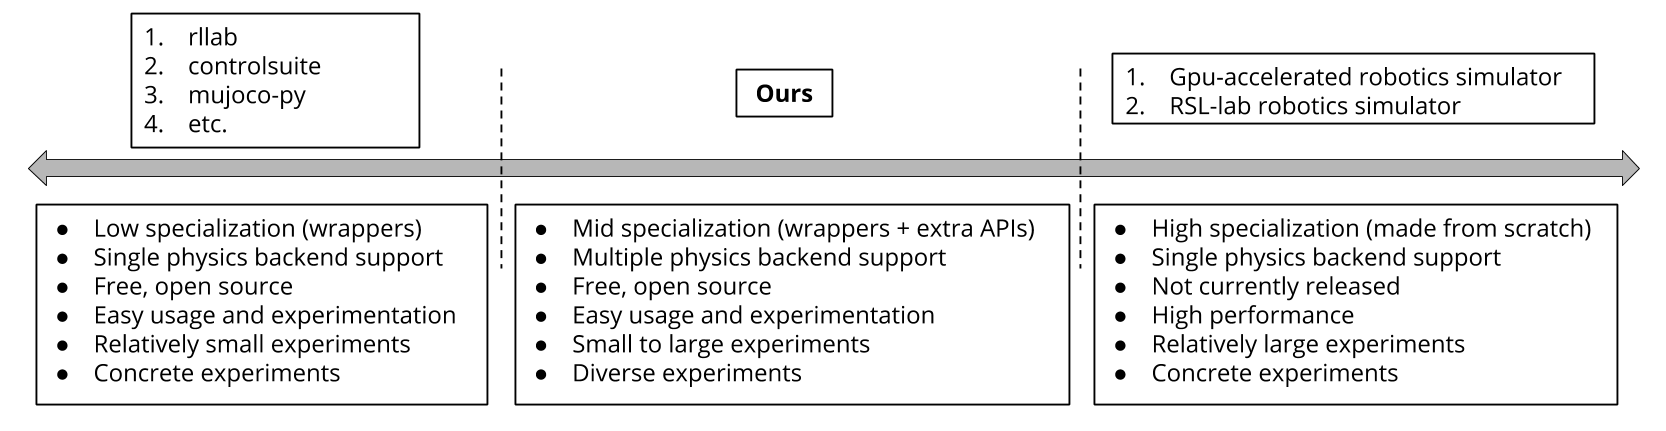
\includegraphics[width=1.0\textwidth]{./chapters/chapter_4/imgs/img_proposal_comparison.png}
        \caption{A comparison of our proposal with currently available benchmarks.}
        \label{fig:ch4_proposal_comparison}
    \end{figure}
}

This thesis is related to the implementation of a \textbf{framework for continuous control
tasks}, with the goal to develop new rich and complex environments, and to create some 
reinforcement learning agents that work in these new environments. 
The first core part is mostly related to the implementation of the \textbf{tools and underlying
infrastructure} of the framework, which so far consists of the following components:

\begin{enumerate}
    \item \textbf{Model creation} tools : to create, visualize, and test a custom model easily.
    \item \textbf{Environment creation} tools : to create, visualize, and test custom environments.
    \item \textbf{Runtime} API : to interact with the user code (agent implementation) and the underlying physics/rendering engines.
    \item \textbf{Python API} : to enable users to easily use the underlying infrastructure and their favourite Deep Learning framework.
\end{enumerate}

The second core part is related to the implementation of the \textbf{reinforcement learning algorithms}
that try to solve the tasks defined by these new complex environments. These algorithms (baselines) will be implemented
using current state-of-the-art algorithms that solve current simple locomotion tasks, and will be evaluated
accordingly. The proposal is depicted in the following figure, where the two core parts are shown. An extra
component is shown to described the future work planned after the completion of this thesis.

\begin{figure}
    \centering
    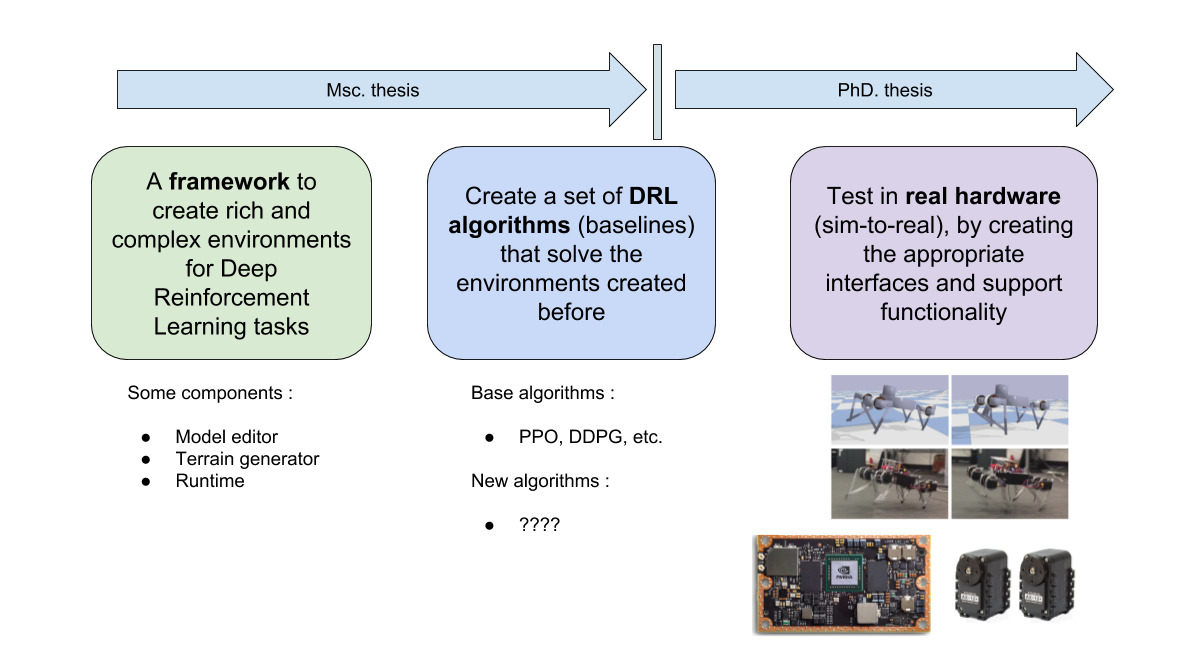
\includegraphics[width=6in]{./chapters/imgs/img_proposal.png}
    \caption[img_proposal]{Proposal and its components}
    \label{fig:img_proposal}
\end{figure}

In this chapter we explain each of these proposed key parts, starting with a description of the proposed 
framework in section 3.1, and then describing the baselines in section 3.2.

\section{Framework and tools}

The proposed framework consists of a set of tools for the creation and usage of complex environments, which
will then be used later for evaluating Deep Reinforcement Learning algorithms. The overall architecture and 
the dependecies to be made are depicted in the following figure, and a brief description of the architecture
would be :

\begin{itemize}
    \item \textbf{An abstract implementation} of the underlying tools, which consists of all the components shown
        in green. This is made abstract in order to make it easy to use with different physics backends and rendering
        backends.
    \item \textbf{A set of adapters} that implement the functionality needed to consume the abstract implementation
        in each specific backend instance, like using Bullet or MuJoCo as engines, or using a custom or third-party
        rendering engine. These consist of the all blue components on top of the abstract dependencies.
    \item \textbf{A set of Python bindings} on top of each specific implementation. These are the APIs to be used
        by the user, and consist of the two purple components.
    \item \textbf{A set of intterfaces} to allow the integration of the before mentioned Python APIs into current
        RL frameworks used by the community.
\end{itemize}

\begin{sidewaysfigure}
    \centering
    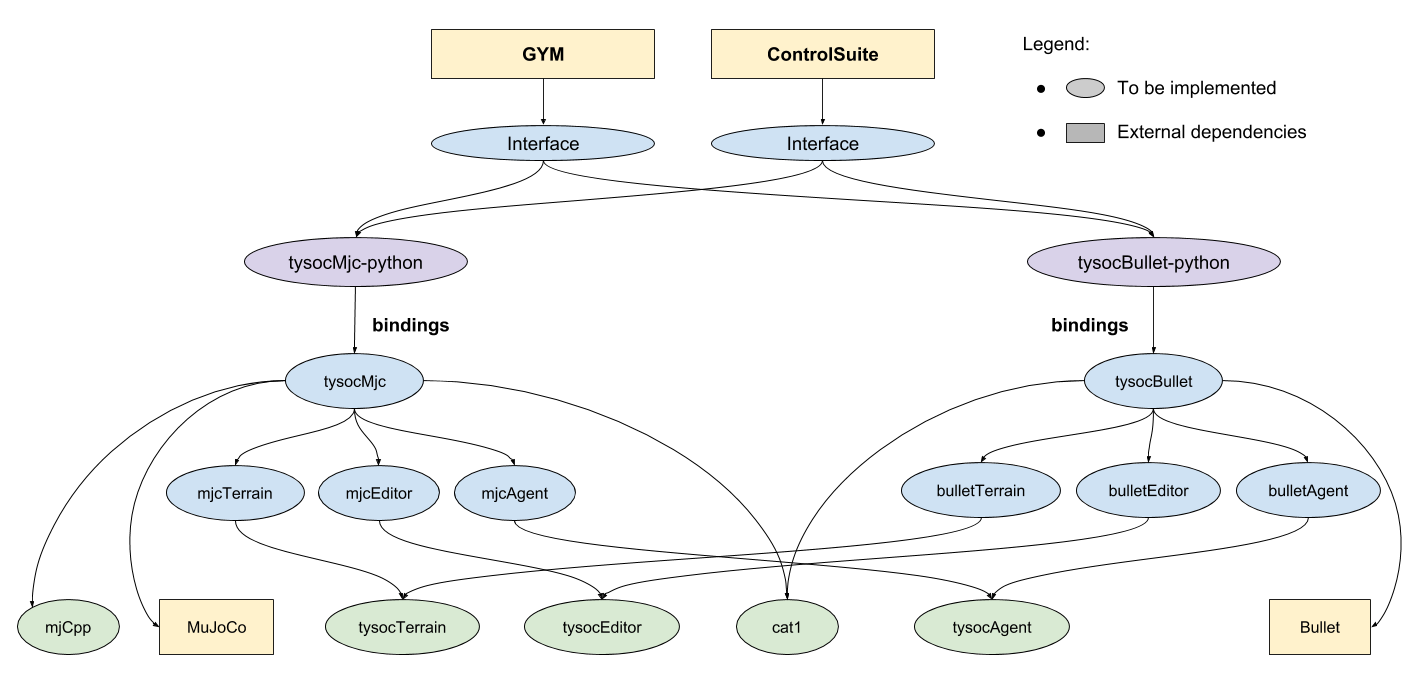
\includegraphics[width=8in]{./chapters/imgs/img_proposal_part1_framework.png}
    \caption[img_proposal_part1_framework]{Overview of the framework architecture}
    \label{fig:img_proposal_part1_framework}
\end{sidewaysfigure}

\section{Baselines}

The proposed baselines consist of various implementations of state-of-the-art Deep Reinforcement Learning
algorithms. We plan on using algorithms like PPO, and DDPG in these environment and evaluate their performances.
According to the literature, there have been tests in more a bit more complex environments (like mazes), but
the results show that current state-of-the-art algorithms can not solve the tasks completely. In this scenarios
is necessary to use different approaches like Hierarchical Reinforcement Learning in order to be able to solve them.
We plan on evaluating as many aspects of the agents as possible in order to gain some insights about the right
direction to take in order to propose improvements that can be made for future works in these environments.

\figProposalComparison